\documentclass[a4paper]{article}    % define document layout
%\documentclass[draft]{article}     % use draft option in packages
%-----------------------------
% preamble
%-----------------------------
\usepackage[sumlimits,]{amsmath}    % math equations and formulas
\usepackage[utf8]{inputenc}         % use UTF-8 encoding
\usepackage[english]{babel}         % use English language
\usepackage{graphicx}              % insert images
%\usepackage[draft]{graphicx}        % do not render figures
\usepackage{subcaption}             % multiple images in one figure
\usepackage{hyperref}               % hyperlinks
\usepackage{float}                  % floating objects (figures, tables)
\usepackage{geometry}               % page size and margins
\geometry{a4paper, margin=1in}      % margins
\usepackage{ragged2e}               % text alignment
\usepackage[table]{xcolor}          % change cell color in tables
%\usepackage{multirow}               % merge rows in table

\graphicspath{                      % path for figures
    {../figures/} 
}

%-----------------------------
% body
%-----------------------------
\begin{document}

\begin{figure}
    \centering
    % UNICAMP logo
    \begin{subfigure}{0.45\textwidth}
        \centering
        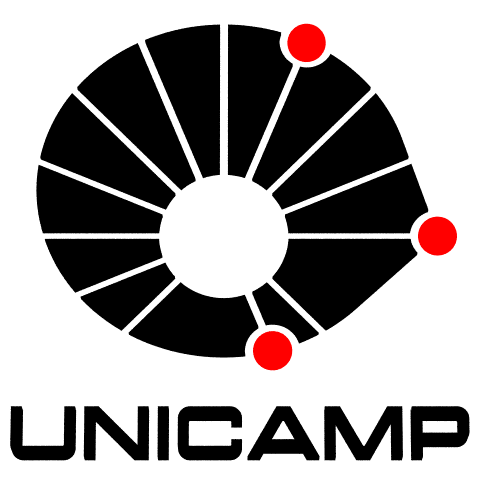
\includegraphics[width=1.5cm]{unicamp}
%        \label{fig:unicamp}
    \end{subfigure}
    \hfill
    % FEEC logo
    \begin{subfigure}{0.45\textwidth}
        \centering
        
\includegraphics[width=1.5cm]{feec}
%        \label{fig:feec}
    \end{subfigure}
\end{figure}

\title{
    \vspace{5cm}
    IA353A - Neural Networks\\
    EC1
    \vspace{1cm}
}
\author{
    Rafael Claro Ito\\
    (R.A.: 118430)
    \vspace{11cm}
}
%R.A.: 118430
%ito.rafael@gmail.com
\date{May 2020}
\maketitle
\newpage

%=================================================
\section*{Questão 1}
%=================================================

%=================================================
\section*{Questão 2}
%=================================================

%=================================================
\section*{Questão 3}
%=================================================

%=================================================
\section*{Questão 4}
%=================================================

%=================================================
\section*{Questão 5}
%=================================================

%=================================================
\section*{Questão 6}
%=================================================

\end{document}
